\documentclass[11pt, xcolor={dvipsnames}, usepdftitle=false]{beamer}
\usepackage{presentation}
\usepackage[brazil]{babel}
\usepackage[utf8]{inputenc}
\usepackage{graphicx}
\hypersetup{pdfpagemode=UseNone, hidelinks, pdfdisplaydoctitle=true,%
pdftitle={Reserva de Salas: Apresentação de Banca Final}}

\input{../../../out/drive-links.tex}

\title{Reserva de Salas}
\author{José Ronaldo dos Santos Júnior}
\date{Londrina, novembro de 2026}

\begin{document}

% ---- Capa ----
% Segue a capa institucional do modelo: logo, nome do sistema, título do trabalho e a
% relação de coordenadores.
\begin{frame}[plain, t]

\includegraphics[width=0.24\textwidth]{../relatorio-estagio/logo-unifil.pdf}
\vspace{4mm}

{\usebeamerfont{title}\usebeamercolor[fg]{title}\MakeLowercase{\inserttitle}\par}
{\color{BlackGray}\rule{\textwidth}{1.5pt}\par}
\vspace{1mm}
{\large Estágio Supervisionado\par}
\vspace{6mm}

{\footnotesize
\begin{flushleft}
\textbf{Aluno:} José Ronaldo dos Santos Júnior\\[1mm]
\textbf{Curso:} Bacharelado em Ciência da Computação\\[1mm]
\textbf{Orientador:} Prof.\ Gustavo Queiroz Silveira\\[1mm]
\textbf{Coordenador Geral:} Prof.\ Dr.\ Sérgio Akio Tanaka\\[1mm]
\textbf{Coordenadora Adjunta Cursos Presenciais:} Profa.\ Ms.\ Simone Sawassaki Tanaka\\[1mm]
\textbf{Coordenadora Adjunta Cursos EaD:} Profa.\ Ms.\ Tânia Camila Kochmanskcy Goulart\\[1mm]
\textbf{Coordenador de Estágio:} Prof.\ Esp.\ Marcelo Yukio Yamamoto
\end{flushleft}}
\vfill
{\centering\insertdate\par}
\end{frame}

% ---- Objetivos e Motivações: os objetivos ----
\begin{frame}
\frametitle{Objetivos e Motivações}
\textbf{Objetivos principais do sistema:}
\begin{itemize}
\item Substituir o gerenciamento atual de salas, feito em planilhas e controle manual
\item Centralizar as informações de agendamento em um só lugar
\item Automatizar o fluxo de solicitação e aprovação de reservas
\item Gerar relatórios de ocupação a partir da agenda consolidada
\end{itemize}
\vspace{3mm}
\textbf{Objetivo de formação:} explorar e aplicar, na prática, conceitos de engenharia de software, do levantamento de requisitos à modelagem e à organização do código.
\end{frame}

% ---- Tecnologias ----
\begin{frame}
\frametitle{Tecnologias Utilizadas}
\begin{itemize}
\item \textbf{Linguagens de Programação:}
\begin{itemize}
\item \textit{Back-end}: Java
\item \textit{Front-end}: JavaScript
\end{itemize}
\item \textbf{Banco de Dados:} PostgreSQL
\item \textbf{Frameworks de Desenvolvimento:}
\begin{itemize}
\item \textit{Front-end}: React
\item \textit{Back-end}: Spring Boot
\end{itemize}
\end{itemize}
\end{frame}

% ---- Separador: Diagramas ----
\begin{frame}
\heading{Modelagem do Sistema}
\end{frame}

% ---- Workflow AS-IS ----
\begin{frame}
\frametitle{Workflow AS-IS (BPMN)}
\begin{figure}
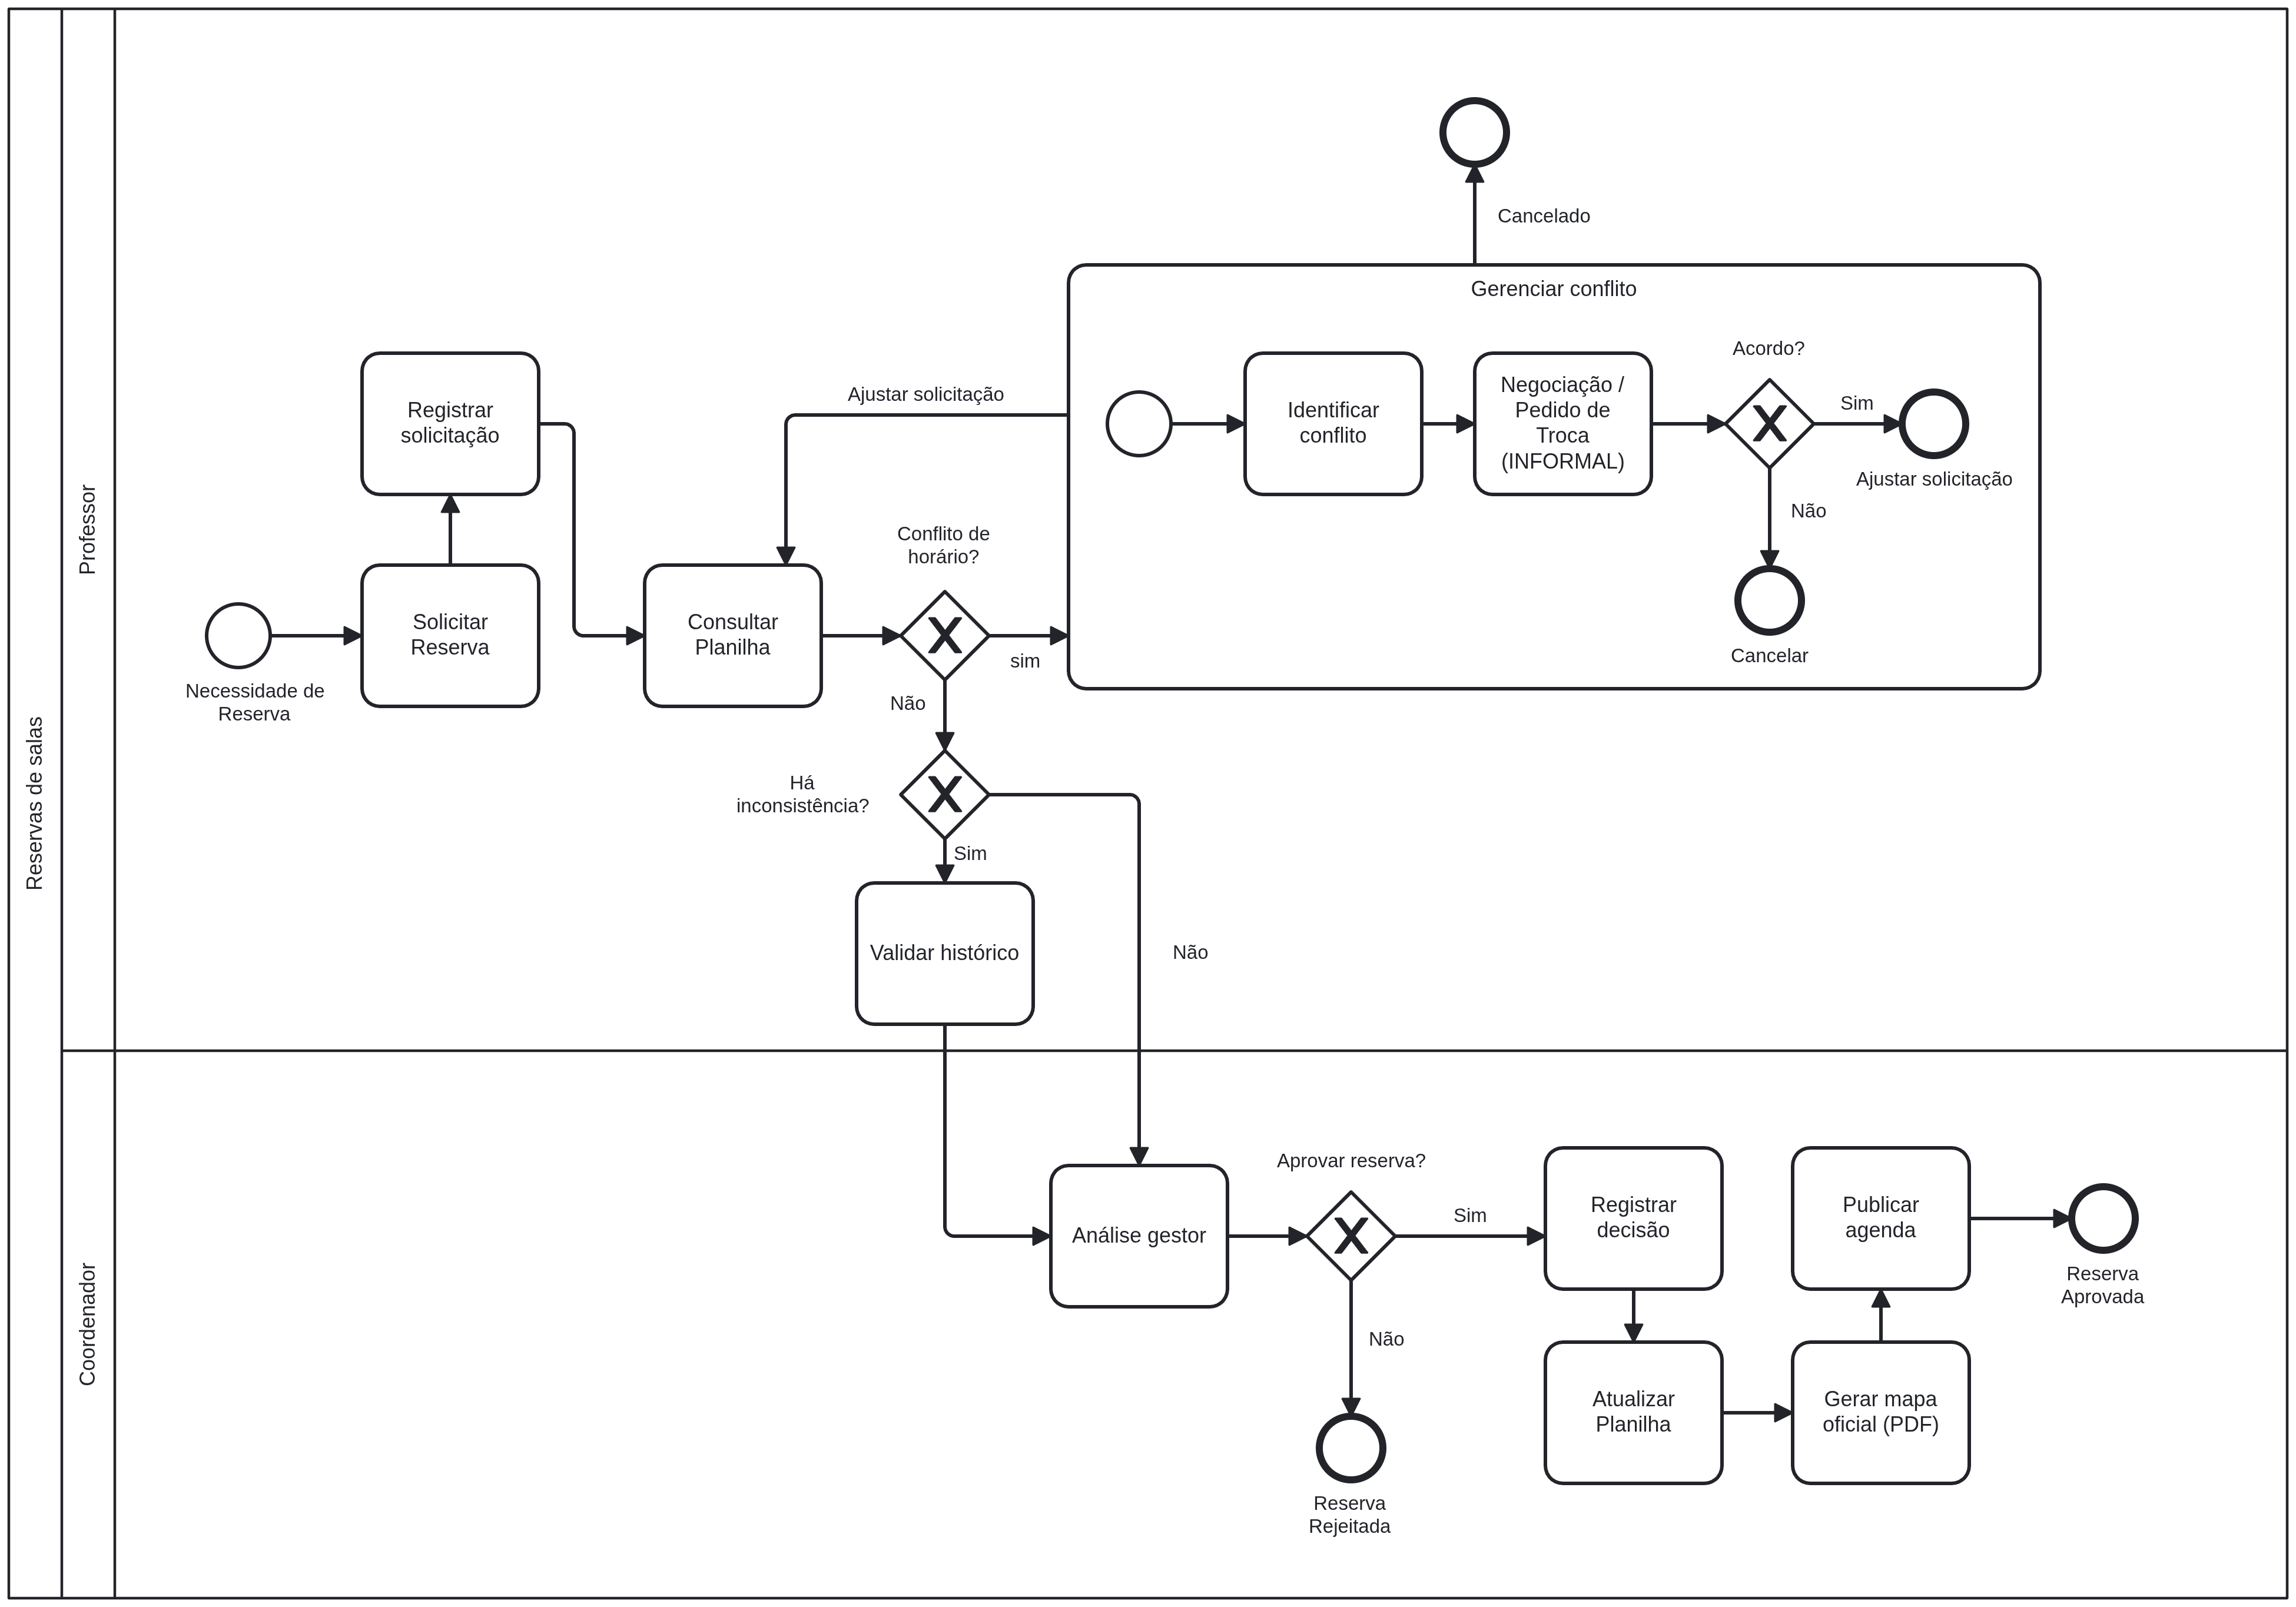
\includegraphics[width=\textwidth,height=0.62\textheight,keepaspectratio]{../relatorio-estagio/imagens/workflow-as-is.png}
\end{figure}
\end{frame}

% ---- Workflow TO-BE ----
\begin{frame}
\frametitle{Workflow TO-BE (BPMN)}
\begin{figure}
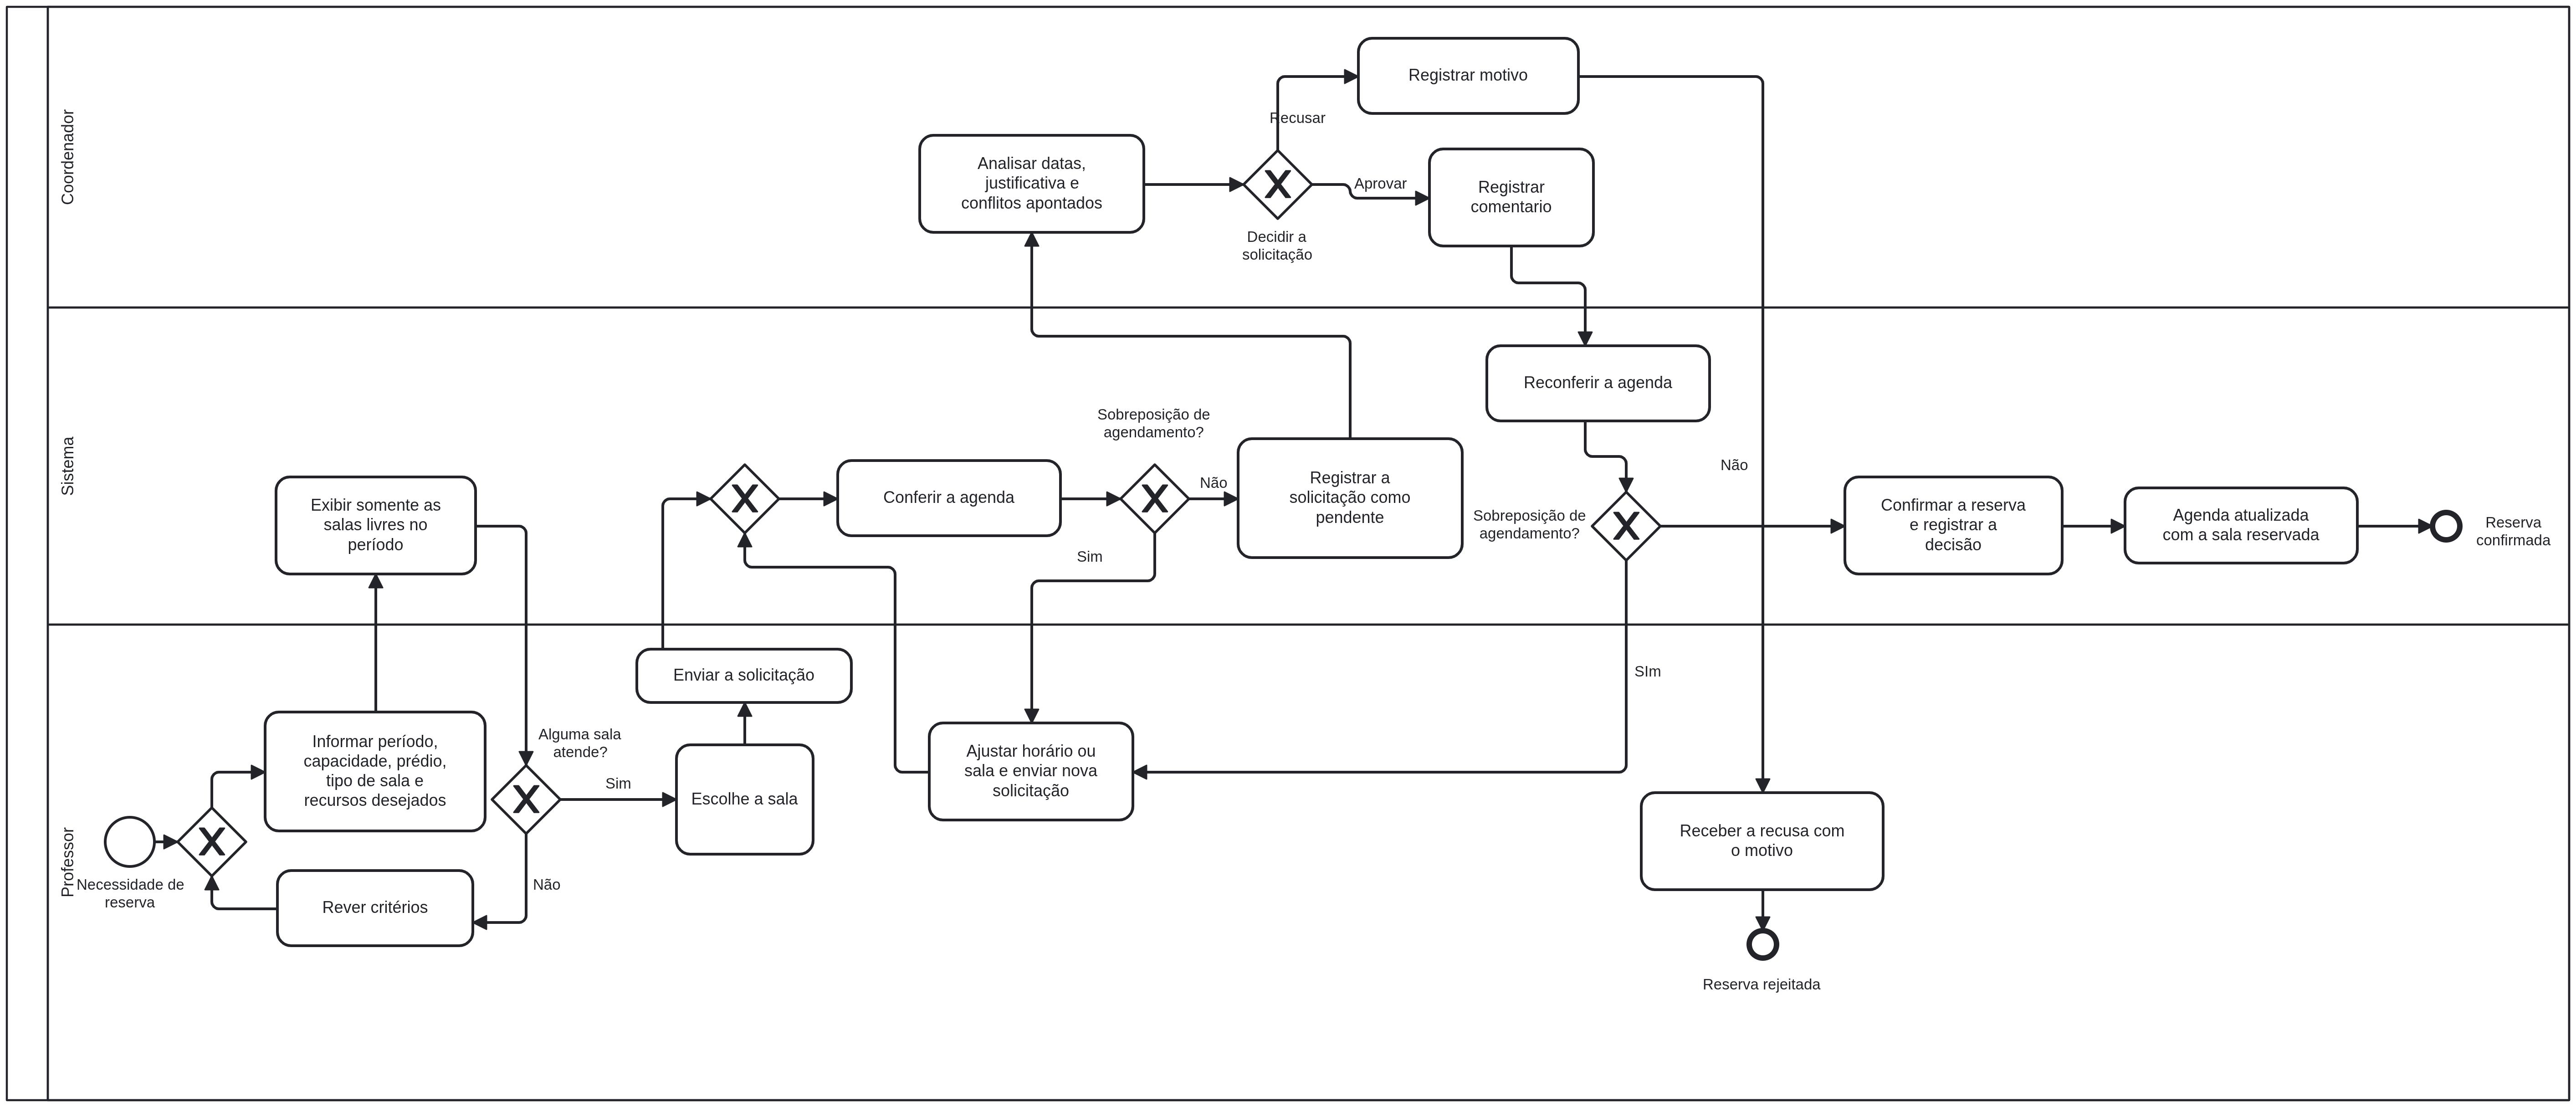
\includegraphics[width=\textwidth,height=0.62\textheight,keepaspectratio]{../relatorio-estagio/imagens/workflow-to-be.png}
\end{figure}
\end{frame}

% ---- Caso de Uso: diagrama ----
\begin{frame}
\frametitle{Diagrama de Caso de Uso}
\begin{figure}
\includegraphics[width=\textwidth,height=0.74\textheight,keepaspectratio]{../../../out/src/plantuml/usecasediagram.png}
\end{figure}
\end{frame}

% ---- Caso de Uso: leitura ----
\begin{frame}
\frametitle{Diagrama de Caso de Uso}
Foram mapeados dez casos de uso no sistema. Entre os principais estão:
\begin{itemize}
\item \textbf{Gerenciar ambientes}, que generaliza o cadastro de prédios, salas, tipos de sala e recursos
\item \textbf{Gerenciar solicitações}, o pedido de alteração da agenda e a sua análise
\item \textbf{Gerenciar agendamentos}, a agenda propriamente dita
\item \textbf{Gerenciar usuários}, exclusivo do coordenador
\end{itemize}
\vspace{3mm}
São dois atores: \textbf{sa\_professor}, o usuário comum, e \textbf{sa\_coordenador}, uma especialização que herda todas as permissões do professor e ganha o gerenciamento de usuários.
\end{frame}

% ---- DER: diagrama ----
\begin{frame}
\frametitle{Modelagem do Banco de Dados}
\begin{figure}
\includegraphics[width=\textwidth,height=0.74\textheight,keepaspectratio]{../../../out/src/plantuml/entidade-relacionamento/der-horizontal.png}
\end{figure}
\end{frame}

% ---- DER: entidades principais ----
\begin{frame}
\frametitle{Modelagem do Banco de Dados}
\textbf{As entidades principais:}
\begin{itemize}
\item \texttt{events}: a reserva em si. Somente eventos aprovados são escritos nesta tabela, que pode ser considerada a agenda do sistema
\item \texttt{event\_requests}: uma solicitação de alteração na agenda
\item \texttt{event\_change\_items}: o conteúdo da mudança, seja a criação de novos eventos, a alteração ou a exclusão
\end{itemize}
\vspace{3mm}
Em volta delas estão as entidades de cadastro, \texttt{users}, \texttt{buildings}, \texttt{rooms}, \texttt{room\_types} e \texttt{resources}, e as de apoio, \texttt{approvals}, \texttt{periods} e \texttt{reports}.
\end{frame}

% ---- Classes: módulos ----
\begin{frame}
\frametitle{Diagrama de Classes}
\begin{columns}[c]
\begin{column}{0.52\textwidth}
\small
O sistema é organizado em módulos separados por domínios específicos.
\vspace{3mm}

Um domínio não deve ter acesso a recursos de outro domínio sem um contrato bem definido, mantendo as suas fronteiras bem definidas.
\end{column}
\begin{column}{0.48\textwidth}
\includegraphics[width=\textwidth,height=0.7\textheight,keepaspectratio]{../../../out/src/plantuml/componentes.png}
\end{column}
\end{columns}
\end{frame}

% ---- Classes: camadas ----
\begin{frame}
\frametitle{Diagrama de Classes}
\begin{columns}[c]
\begin{column}{0.44\textwidth}
\small
Cada módulo é dividido em camadas menores, com o seu próprio domínio, os seus casos de uso e a sua camada de infraestrutura.
\vspace{3mm}
\begin{itemize}
\item \textbf{Domain}: entidades, objetos de valor e enumerações
\item \textbf{Application}: casos de uso e portas
\item \textbf{Infrastructure}: controladores, repositórios e adaptadores
\end{itemize}
\end{column}
\begin{column}{0.56\textwidth}
\includegraphics[width=\textwidth,height=0.82\textheight,keepaspectratio]{../../../out/src/plantuml/classe/simples/camadas.png}
\end{column}
\end{columns}
\end{frame}

% ---- Classes: um diagrama por módulo ----
% Versões simplificadas (classe/simples/), que cortam DTOs, mappers, validators,
% getters e construtores. As exaustivas estão em classe/<modulo>.puml.
\begin{frame}
\frametitle{Diagrama de Classes: Módulo de Usuários}
\begin{figure}
\includegraphics[width=\textwidth,height=0.82\textheight,keepaspectratio]{../../../out/src/plantuml/classe/simples/user_simples.png}
\end{figure}
\end{frame}

\begin{frame}
\frametitle{Diagrama de Classes: Módulo de Salas}
\begin{figure}
\includegraphics[width=\textwidth,height=0.82\textheight,keepaspectratio]{../../../out/src/plantuml/classe/simples/room/room_room.png}
\end{figure}
\end{frame}

\begin{frame}
\frametitle{Diagrama de Classes: Módulo de Eventos}
\begin{figure}
\includegraphics[width=\textwidth,height=0.82\textheight,keepaspectratio]{../../../out/src/plantuml/classe/simples/event/event_and_request.png}
\end{figure}
\end{frame}

\begin{frame}
\frametitle{Diagrama de Classes: Módulo de Relatórios}
\begin{figure}
\includegraphics[width=\textwidth,height=0.82\textheight,keepaspectratio]{../../../out/src/plantuml/classe/simples/report_simples.png}
\end{figure}
\end{frame}

% ---- Classes: a porta ----
\begin{frame}
\frametitle{Diagrama de Classes}
\begin{columns}[c]
\begin{column}{0.44\textwidth}
\small
\textbf{Exemplo:} o módulo de relatórios precisa de informações que pertencem ao módulo de salas para conseguir gerar os seus relatórios.
\vspace{3mm}

Na sua camada de aplicação, ele expõe uma interface que é o contrato que espera, no caso \texttt{RoomReportDataPort}.
\end{column}
\begin{column}{0.56\textwidth}
\includegraphics[width=\textwidth,height=0.8\textheight,keepaspectratio]{../../../out/src/plantuml/classe/simples/contrato_modulos.png}
\end{column}
\end{columns}
\end{frame}

% ---- Classes: o adaptador ----
\begin{frame}
\frametitle{Diagrama de Classes}
\begin{columns}[c]
\begin{column}{0.44\textwidth}
\small
Na camada de infraestrutura, agora do módulo de salas, implementamos essa interface, fechando o contrato entre os dois módulos.
\vspace{3mm}

O módulo de relatórios depende da porta, não do módulo de salas. Nenhum dos dois conhece as classes internas do outro.
\end{column}
\begin{column}{0.56\textwidth}
\includegraphics[width=\textwidth,height=0.8\textheight,keepaspectratio]{../../../out/src/plantuml/classe/simples/contrato_modulos.png}
\end{column}
\end{columns}
\end{frame}

% ---- Estado: a pergunta ----
\begin{frame}
\frametitle{Diagrama de Estado}
\begin{columns}[c]
\begin{column}{0.56\textwidth}
\small
Os diagramas de estado representam os possíveis estados que uma entidade poderá ter no banco de dados.
\vspace{4mm}

Como o sistema garante que uma entidade excluída não saia deste estado?
\end{column}
\begin{column}{0.44\textwidth}
\includegraphics[width=\textwidth,height=0.72\textheight,keepaspectratio]{../../../out/src/plantuml/estado/user_status.png}
\end{column}
\end{columns}
\end{frame}

% ---- Estado: a resposta ----
\begin{frame}
\frametitle{Diagrama de Estado}
\begin{columns}[c]
\begin{column}{0.40\textwidth}
\small
Cada transição de estado é uma operação específica, e essas operações estão na camada de domínio, isto é, no núcleo do sistema.
\vspace{3mm}

Para excluir um usuário, executamos a operação de excluir usuário e só então salvamos no banco. Não há edição livre do campo, e portanto não há margem para entidades em estado inválido no futuro.
\end{column}
\begin{column}{0.60\textwidth}
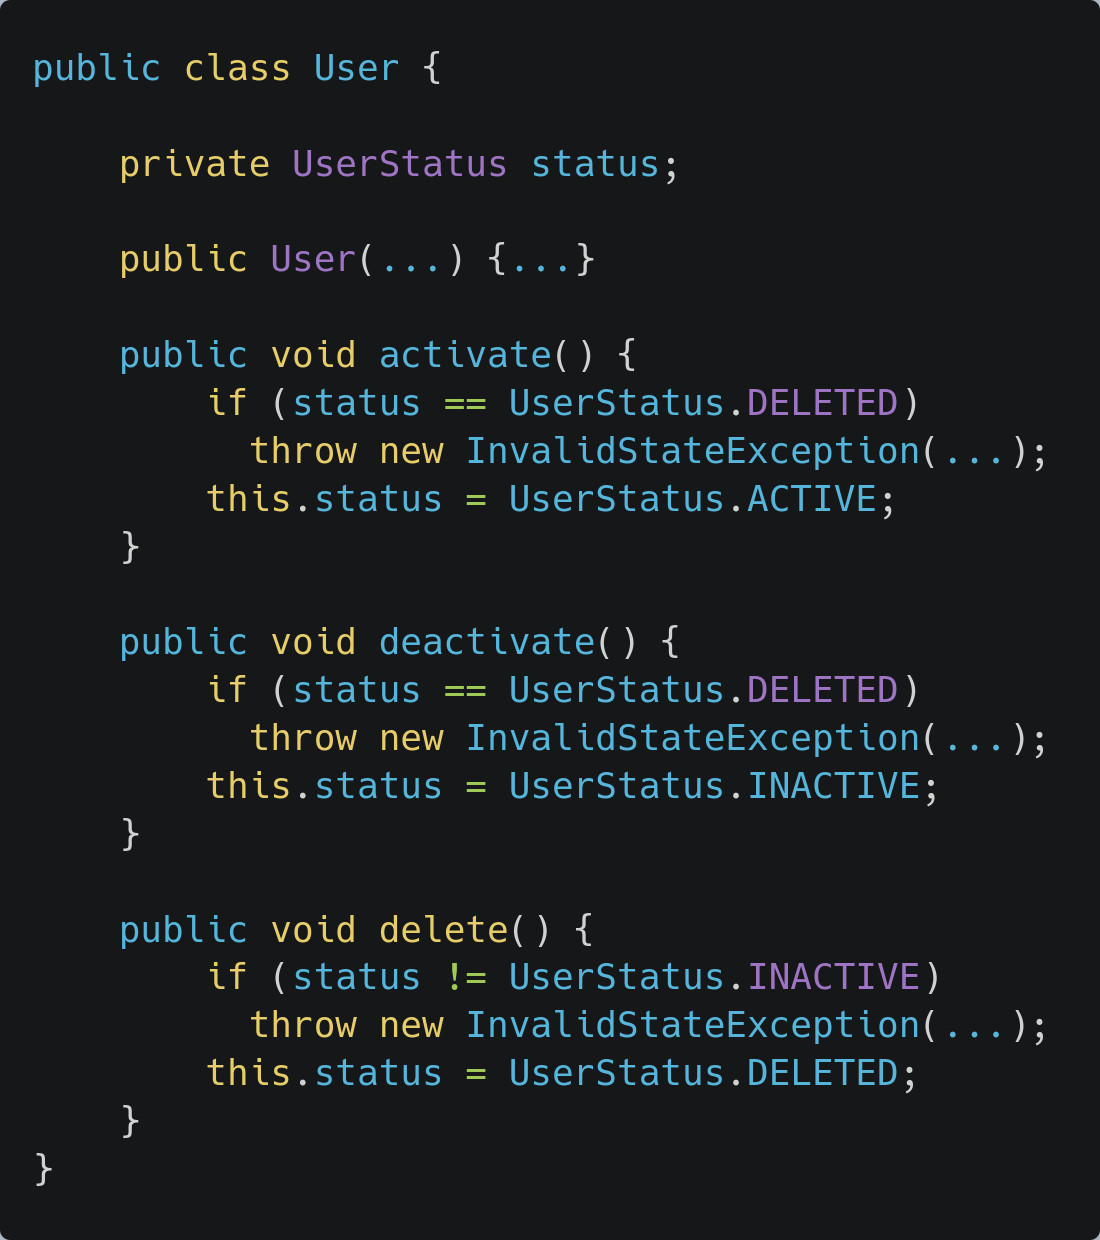
\includegraphics[width=\textwidth,height=0.82\textheight,keepaspectratio]{user-example.png}
\end{column}
\end{columns}
\end{frame}

% ---- Sequência: módulo de usuários ----
% Versão simplificada (sequencia/simples/user.puml): só o caminho de sucesso, com a
% camada de casos de uso e a de repositórios como raias. Os cinco diagramas por
% endpoint estão em sequencia/user/.
\begin{frame}
\frametitle{Diagrama de Sequência: Módulo de Usuários}
\begin{figure}
\includegraphics[width=\textwidth,height=0.82\textheight,keepaspectratio]{../../../out/src/plantuml/sequencia/simples/user_simples.png}
\end{figure}
\end{frame}

% ---- Diagrama de Implantação ----
\begin{frame}
\frametitle{Diagrama de Implantação}
\begin{figure}
\includegraphics[width=\textwidth,height=0.72\textheight,keepaspectratio]{../../../out/src/plantuml/deployment.png}
\end{figure}
\end{frame}

% ---- Separador: Sistema ----
\begin{frame}
\heading{Apresentação do Sistema}
\end{frame}

% ---- Demonstração ----
\begin{frame}
\frametitle{Demonstração}
\begin{itemize}
\item Login e autenticação
\item Cadastro e gerenciamento de salas, com tipo, capacidade e recursos
\item Busca de salas disponíveis
\item Solicitação e acompanhamento de reservas
\item Grade de horários e ocupação das salas
\end{itemize}
\end{frame}

% ---- Artefatos de Requisitos ----
\begin{frame}
\frametitle{Artefatos de Requisitos}
\begin{itemize}
\item \textbf{Documento de Visão}
\item \textbf{Especificação Complementar}
\item \textbf{Glossário}
\item \textbf{Solicitação dos Principais Envolvidos}
\item \textbf{Especificação de Caso de Uso}
\end{itemize}
\end{frame}

\begin{frame}
\frametitle{Conceitos de Engenharia de Software Aplicados}
\begin{itemize}
\item \textbf{Clean Architecture (Ports \& Adapters):} domínio, aplicação e infraestrutura separados; portas implementadas por adaptadores
\item \textbf{Domain-Driven Design:} entidades ricas em comportamento, value objects para os identificadores e agregados referenciados por ID
\item \textbf{Monólito Modular:} módulos por domínio com núcleo compartilhado, comunicando-se via portas
\end{itemize}
\end{frame}

% ---- Conclusões e Trabalhos Futuros ----
\begin{frame}
\frametitle{Conclusões e Trabalhos Futuros}
\textbf{Conclusões:}
\begin{itemize}
\item Foi possível aplicar na prática conceitos estudados em sala: levantamento de requisitos, mapeamento de processos em BPMN e modelagem de sistemas
\item O maior desafio foi gerenciar a complexidade do software: definir as fronteiras entre os módulos e separar a regra de negócio do detalhe de tecnologia, o que levou a organizar a aplicação em camadas com as dependências voltadas para o domínio
\end{itemize}
\end{frame}

\begin{frame}
\frametitle{Conclusões e Trabalhos Futuros}
\textbf{Trabalhos futuros:}
\begin{itemize}
\item Notificações automáticas sobre mudanças no status das solicitações
\item Relatório de grade de horários, consolidando a ocupação ao longo do semestre
\item Solicitação de troca de salas entre professores, trazendo para dentro do sistema a negociação que hoje é informal
\end{itemize}
\end{frame}

\begin{frame}
\heading{Obrigado!}
\end{frame}

\lastslide

\end{document}
